\documentclass[12pt]{article}

% ── Packages ──────────────────────────────────────────────────────────────────
\usepackage[margin=1in]{geometry}
\usepackage{amsmath,amssymb}
\usepackage{graphicx}
\usepackage{booktabs}
\usepackage{hyperref}
\usepackage[numbers]{natbib}
\usepackage{algorithm}
\usepackage{algorithmic}
\usepackage{xcolor}
\usepackage{subcaption}
\usepackage{float}

% convenience command for placeholder figures
\newcommand{\placeholder}[2]{%
  \begin{center}
    \fbox{\parbox{0.85\linewidth}{\centering\vspace{#1}\textcolor{gray}{\small\textit{#2}}\vspace{#1}}}
  \end{center}
}

% ── Title ─────────────────────────────────────────────────────────────────────
\title{\textbf{MPEdit: SDEdit-Style Path Regeneration\\for Motion Planning Diffusion}}
\author{Danny Broyd}
\date{}

\begin{document}
\maketitle

% ══════════════════════════════════════════════════════════════════════════════
% ABSTRACT
% ══════════════════════════════════════════════════════════════════════════════
\begin{abstract}
Diffusion-based motion planners can produce high-quality, collision-free
trajectories, but they plan from scratch each time, discarding any prior
solution.  We present \textbf{MPEdit}, a framework that adapts the
\emph{SDEdit} image-editing paradigm to robot motion planning.  Given an
existing trajectory and a modified obstacle map, MPEdit adds controlled noise
to the trajectory's B-spline control points and denoises under an updated
collision-cost guide, yielding a new collision-free path that stays close to
the original.  The same mechanism enables a \emph{sketch-to-path} mode in
which a rough, hand-drawn path is refined into a feasible trajectory.
We build on Motion Planning Diffusion (MPD) and evaluate MPEdit in both 2-D
point-mass and 7-DOF Panda arm environments.  Experiments show that MPEdit
achieves competitive success rates while producing paths that are
significantly more faithful to the original trajectory than replanning from
scratch, at comparable or faster inference times.
\end{abstract}

% ══════════════════════════════════════════════════════════════════════════════
\section{Introduction}
\label{sec:intro}
% ══════════════════════════════════════════════════════════════════════════════

Classical motion planning algorithms such as RRT~\cite{lavalle1998rrt} and
its bi-directional variant RRTConnect~\cite{kuffner2000rrtconnect} can
reliably find collision-free paths, but every invocation starts from scratch.
When the environment changes only slightly---for example, a single obstacle
is added or removed---re-running a planner wastes the information already
embedded in the previous solution.

Recently, \emph{diffusion models} have been applied to motion planning.
Motion Planning Diffusion (MPD)~\cite{carvalho2023mpd} trains a denoising
diffusion model on a dataset of collision-free trajectories represented as
B-spline control points.  At inference time, cost guidance steers the
denoising process away from collisions, producing smooth, high-quality paths.
However, MPD also generates trajectories from pure noise, ignoring any
existing solution.

In image generation, \emph{SDEdit}~\cite{meng2022sdedit} showed that one can
\emph{edit} an existing image by adding noise at an intermediate diffusion
step and then denoising.  The amount of noise controls the trade-off between
fidelity to the input and the model's ability to ``fix'' the image.

We combine these two ideas into \textbf{MPEdit}: given an existing trajectory
and an updated obstacle map, we (1) add noise to the trajectory's B-spline
control points at an intermediate diffusion time-step~$t_0$, and (2) denoise
from~$t_0$ to~$0$ with the collision-cost guide recomputed for the new
environment.  A larger~$t_0$ gives the model more freedom to deviate from the
input, trading faithfulness for a higher success rate.

The same pipeline supports a \emph{sketch-to-path} mode: the user draws a
rough path in configuration space, and the model refines it into a feasible,
smooth trajectory.  We provide interactive GUI tools for both obstacle editing
and path sketching.

We evaluate MPEdit on five experiments covering noise-level trade-offs,
baseline comparisons, sketch-mode quality, inference speed, and output
diversity.  Our results show that MPEdit offers a practical middle ground
between the reliability of sampling-based planners and the data-driven
smoothness of diffusion models.

% ══════════════════════════════════════════════════════════════════════════════
\section{Background}
\label{sec:background}
% ══════════════════════════════════════════════════════════════════════════════

\subsection{Motion Planning Diffusion (MPD)}
\label{sec:mpd}

MPD~\cite{carvalho2023mpd} trains a Gaussian denoising diffusion model on
trajectories represented as B-spline control points.  A trajectory
$\tau = (q_1, \dots, q_T)$ in joint space is parameterized by a vector of
control points~$\mathbf{c}\in\mathbb{R}^{K\times d}$, where $K$ is the
number of control points and $d$ is the configuration-space dimension.  The
forward diffusion process gradually adds Gaussian noise:
\begin{equation}
  q(\mathbf{c}_t \mid \mathbf{c}_0)
    = \mathcal{N}\!\bigl(\sqrt{\bar\alpha_t}\,\mathbf{c}_0,\;
      (1-\bar\alpha_t)\,\mathbf{I}\bigr),
  \label{eq:forward}
\end{equation}
where $\bar\alpha_t = \prod_{s=1}^{t}\alpha_s$ follows a noise schedule.

A neural network $\epsilon_\theta(\mathbf{c}_t, t, \mathbf{z})$ is trained to
predict the noise~$\epsilon$ given the noisy control points~$\mathbf{c}_t$,
the diffusion step~$t$, and context information
$\mathbf{z} = (q_\text{start}, q_\text{goal}, p_\text{EE})$ encoding the
start configuration, goal configuration, and end-effector goal pose.

At inference, reverse diffusion iteratively denoises from
$\mathbf{c}_T \sim \mathcal{N}(0, \mathbf{I})$ back to $\mathbf{c}_0$.
\emph{Cost guidance}~\cite{dhariwal2021diffusion} adds a gradient signal
$-\nabla_{\mathbf{c}_t} \mathcal{J}(\mathbf{c}_t)$ at each step, where
$\mathcal{J}$ aggregates collision costs computed from the signed-distance
field (SDF) of the environment.  This steers the trajectory away from
obstacles without retraining.  MPD uses DDIM~\cite{song2021ddim} sampling for
deterministic, accelerated inference.

\subsection{SDEdit}
\label{sec:sdedit}

SDEdit~\cite{meng2022sdedit} introduces stochastic differential equation
(SDE)--based editing for images.  Instead of denoising from pure noise, one
starts from a \emph{reference} image~$x_0$, adds noise to an intermediate
level~$t_0$, and runs the reverse SDE from~$t_0$ to~$0$.  For small~$t_0$
the output closely follows the input; for large~$t_0$ the model has more
freedom and the result is less faithful but potentially more ``correct''
according to the learned data distribution.  This provides a simple,
training-free mechanism for guided image editing.

\subsection{B-Spline Trajectory Representation}
\label{sec:bspline}

Both MPD and MPEdit represent trajectories using uniform cubic B-splines.  A
small set of $K$ control points fully determines a smooth curve with $T \gg K$
waypoints, reducing the dimensionality of the diffusion model's output space
while guaranteeing $C^2$ continuity.  Hard boundary conditions (start and goal
configurations) are enforced by clamping the first and last control points
after every denoising step.

% ══════════════════════════════════════════════════════════════════════════════
\section{Method}
\label{sec:method}
% ══════════════════════════════════════════════════════════════════════════════

\subsection{SDEdit for Motion Planning}
\label{sec:sdedit_mp}

Given an existing collision-free trajectory~$\tau_\text{ref}$ (e.g., planned
by RRTConnect in the \emph{original} obstacle map) and an updated obstacle
map, MPEdit proceeds as follows:

\begin{enumerate}
  \item \textbf{Convert to control points.}  Map $\tau_\text{ref}$ to
        normalized B-spline control points
        $\mathbf{c}_0 \in \mathbb{R}^{K\times d}$ using least-squares fitting
        and the dataset normalization statistics.
  \item \textbf{Add noise.}  Sample
        $\mathbf{c}_{t_0} \sim q(\mathbf{c}_{t_0}\mid\mathbf{c}_0)$
        using~\eqref{eq:forward} at a user-specified noise level~$t_0$.
  \item \textbf{Denoise with updated cost guide.}  Run DDIM reverse
        diffusion from step~$t_0$ down to~$0$, with the collision-cost guide
        recomputed from the \emph{modified} SDF.  Hard boundary conditions
        are re-applied at every step.
  \item \textbf{Select best path.}  Among the $N$ denoised trajectories,
        discard those that collide with the updated environment and select the
        shortest collision-free path.
\end{enumerate}

The noise level~$t_0$ is the key hyperparameter: it controls the trade-off
between \emph{faithfulness} to the reference path (measured by Fréchet and
L2 distances) and the \emph{success rate} (fraction of collision-free
outputs).  We study this trade-off systematically in
Section~\ref{sec:exp_t0}.

Algorithm~\ref{alg:sdedit} summarizes the MPEdit inference procedure.

\begin{algorithm}[t]
\caption{MPEdit: SDEdit-style path regeneration}
\label{alg:sdedit}
\begin{algorithmic}[1]
\REQUIRE Reference path $\tau_\text{ref}$, noise level $t_0$, modified
         environment SDF, number of samples~$N$
\STATE $\mathbf{c}_0 \gets \textsc{PathToControlPoints}(\tau_\text{ref})$
\STATE $\mathbf{c}_0 \gets \textsc{Normalize}(\mathbf{c}_0)$
\FOR{$i = 1$ \TO $N$}
  \STATE $\epsilon \sim \mathcal{N}(0, \mathbf{I})$
  \STATE $\mathbf{c}_{t_0}^{(i)} \gets \sqrt{\bar\alpha_{t_0}}\,\mathbf{c}_0
         + \sqrt{1 - \bar\alpha_{t_0}}\,\epsilon$
\ENDFOR
\FOR{$t = t_0, t_0{-}1, \dots, 1$}
  \STATE $\hat\epsilon \gets \epsilon_\theta(\mathbf{c}_t, t, \mathbf{z})$
  \STATE $\mathbf{c}_{t-1} \gets \textsc{DDIMStep}(\mathbf{c}_t, \hat\epsilon)
         - \eta\,\nabla_{\mathbf{c}_t}\mathcal{J}_\text{collision}(\mathbf{c}_t)$
  \STATE Clamp start/goal control points
\ENDFOR
\STATE $\mathbf{c}_0 \gets \textsc{Unnormalize}(\mathbf{c}_0)$
\STATE $\mathcal{T} \gets \{\tau^{(i)} \mid \tau^{(i)}
       = \textsc{BSpline}(\mathbf{c}_0^{(i)}),\;
       \text{collision-free}\}$
\RETURN $\arg\min_{\tau\in\mathcal{T}} \textsc{PathLength}(\tau)$
\end{algorithmic}
\end{algorithm}

\subsection{Re-Planning Mode}
\label{sec:replan}

In the re-planning scenario the environment changes after an initial path has
been computed.  Typical modifications include:
\begin{itemize}
  \item \textbf{Adding obstacles:} a new sphere or box is inserted, possibly
        intersecting the current path.
  \item \textbf{Removing obstacles:} an existing obstacle disappears, opening
        shorter routes.
\end{itemize}
After the modification, the SDF is recomputed and the cost guide is rebuilt.
MPEdit then takes the now-invalid reference path, adds noise, and denoises
under the new cost, producing a trajectory that respects the updated map while
staying close to the original route.

We classify obstacle modifications into four difficulty levels:
\textbf{easy} (small obstacle far from the path), \textbf{medium}
(moderate obstacle near the path), \textbf{hard} (large obstacle blocking
the path), and \textbf{removal} (an existing obstacle is removed).

\subsection{Sketch-to-Path Mode}
\label{sec:sketch}

In sketch mode the user draws a rough path from start to goal using an
interactive GUI (see Appendix~\ref{app:sketch}).  The sketch is resampled
to the model's waypoint count via cubic B-spline fitting and then treated
exactly like a reference path: noise is added at level~$t_0$ and the
model denoises it into a feasible trajectory.  Because the sketch may
violate collision constraints or lack smoothness, a higher~$t_0$ is
typically required.  The trade-off is controlled by both~$t_0$ and the
``corruption level''~$\sigma$ that measures how far the sketch deviates
from a legal path.

% ══════════════════════════════════════════════════════════════════════════════
\section{Experimental Setup}
\label{sec:experiments}
% ══════════════════════════════════════════════════════════════════════════════

\paragraph{Environments.}
We evaluate on two environments:
\begin{itemize}
  \item \textbf{EnvSimple2D--PointMass2D:} a 2-D workspace with circular
        obstacles and a point-mass robot ($d{=}2$).
  \item \textbf{EnvSpheres3D--Panda:} a 3-D workspace with spherical
        obstacles and a 7-DOF Franka Emika Panda arm ($d{=}7$).
\end{itemize}

\paragraph{Baselines.}
We compare three methods:
\begin{itemize}
  \item \textbf{SDEdit (ours):} MPEdit with noise level $t_0{=}7$
        (tuned via Experiment~1).
  \item \textbf{Full MPD:} standard MPD inference from pure noise ($t_0{=}0$,
        i.e.\ the full diffusion schedule).
  \item \textbf{RRTConnect:} classical bi-directional RRT with a 10\,s
        time limit.
\end{itemize}

\paragraph{Metrics.}
\begin{itemize}
  \item \textbf{Success rate (S\%):} fraction of collision-free paths out of
        $N{=}100$ samples.
  \item \textbf{Discrete Fréchet distance:} maximum pointwise distance along
        the optimal alignment between the regenerated and input paths
        (lower~$=$~more faithful).
  \item \textbf{Mean L2 distance:} mean per-waypoint Euclidean distance
        after arc-length resampling.
  \item \textbf{Inference time:} wall-clock seconds on a single NVIDIA GPU.
  \item \textbf{Path length} and \textbf{smoothness:} standard trajectory
        quality measures.
  \item \textbf{Pairwise diversity:} mean pairwise Fréchet distance among all
        generated trajectories (higher~$=$~more diverse).
\end{itemize}

\paragraph{Protocol.}
Each experiment uses 50 start--goal pairs drawn from the validation set, with
100 trajectory samples per pair.  All runs use seed~42 for reproducibility.
Experiments are configured via YAML files and executed by a unified experiment
runner.

% ══════════════════════════════════════════════════════════════════════════════
\section{Results}
\label{sec:results}
% ══════════════════════════════════════════════════════════════════════════════

\subsection{Experiment 1: Noise-Level Trade-Off ($t_0$ Sweep)}
\label{sec:exp_t0}

We sweep the noise level $t_0 \in \{1, 2, \dots, 14\}$ on the medium
difficulty scenario and plot success rate and Fréchet distance.
Figure~\ref{fig:t0_sweep} shows the expected trade-off: low~$t_0$ yields
high faithfulness but low success, while high~$t_0$ increases success at the
cost of diverging from the reference.  The ``elbow'' around $t_0{=}7$
offers a good balance and is used in subsequent experiments.

\begin{figure}[t]
  \centering
  % Replace with: 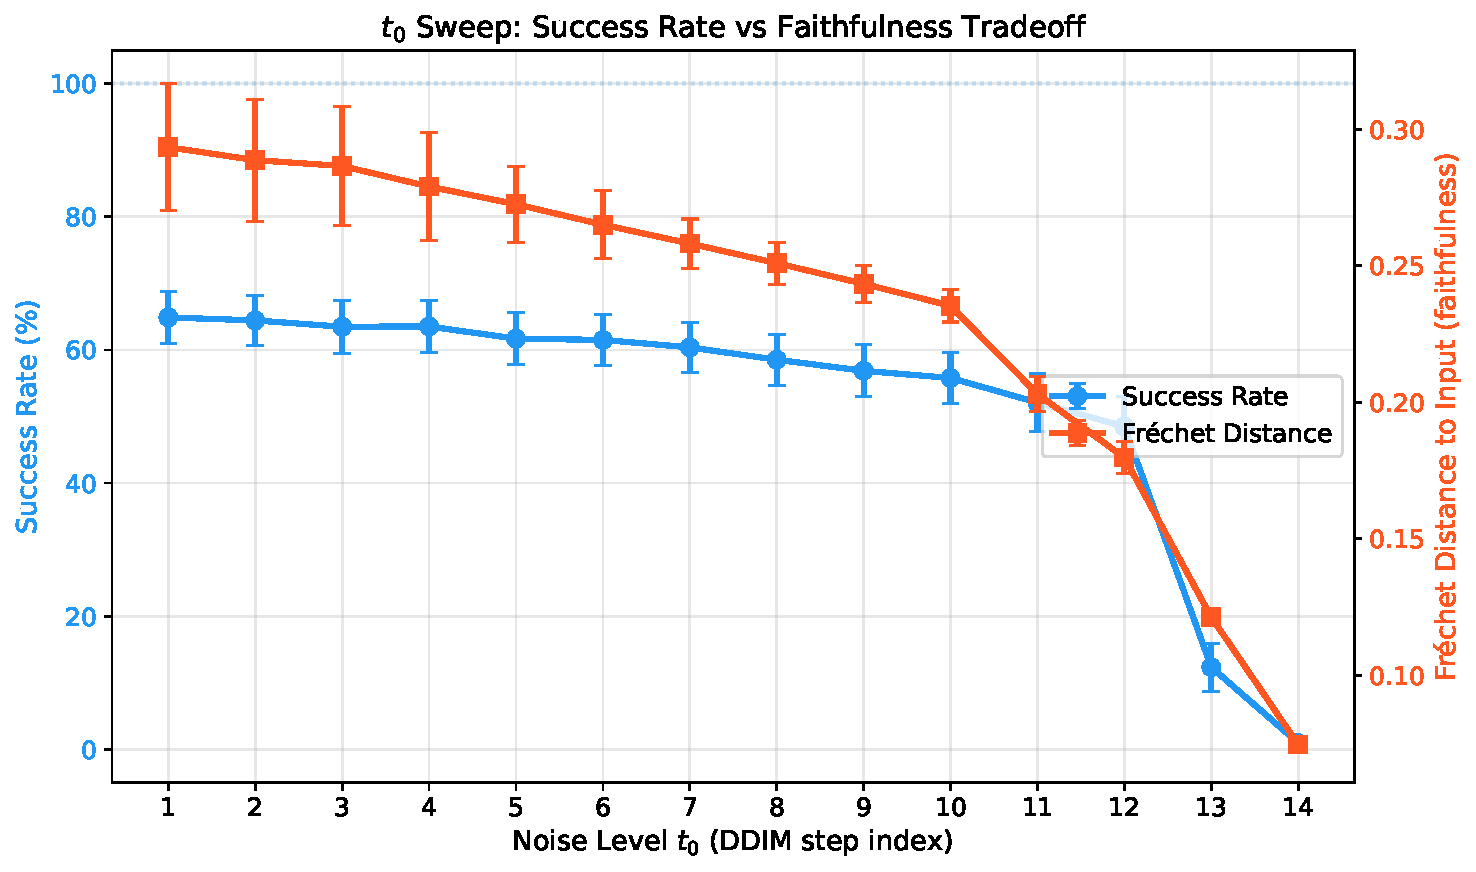
\includegraphics[width=\linewidth]{../scripts/inference/logs_experiments/figures/fig2_t0_sweep.pdf}
  \placeholder{1cm}{Figure~2: Noise-level sweep ($t_0 = 1 \ldots 14$).
    Left axis: success rate (\%).  Right axis: Fréchet distance to input path.}
  \caption{Noise-level trade-off.  Success rate (left axis, \%) increases
    with $t_0$, while faithfulness measured by Fréchet distance (right axis)
    decreases.}
  \label{fig:t0_sweep}
\end{figure}

\subsection{Experiment 2: Baseline Comparison}
\label{sec:exp_baselines}

Table~\ref{tab:baselines} compares SDEdit ($t_0{=}7$), Full MPD, and
RRTConnect across the four difficulty scenarios on the 3-D Panda environment.

\begin{table}[t]
\centering
\caption{Re-planning comparison across difficulty scenarios
  (EnvSpheres3D--Panda, 50 pairs $\times$ 100 samples).}
\label{tab:baselines}
\begin{tabular}{llrrrrrr}
\toprule
Scenario & Method & S\% & Fréchet$\downarrow$ & L2$\downarrow$
  & Time(s)$\downarrow$ & PathLen & Smooth \\
\midrule
easy & SDEdit      & 89.3\% & 0.146 & 0.070 & 0.659 & 1.835 & 0.000 \\
easy & Full MPD    & 86.9\% & 0.187 & 0.090 & 0.780 & 1.830 & 0.000 \\
easy & RRTConnect  & 100.0\% & 0.171 & 0.087 & 0.311 & 1.776 & 0.000 \\
\midrule
medium & SDEdit    & 49.2\% & 0.261 & 0.111 & 0.745 & 1.942 & 0.000 \\
medium & Full MPD  & 52.7\% & 0.282 & 0.125 & 0.861 & 1.937 & 0.000 \\
medium & RRTConnect& 100.0\% & 0.422 & 0.215 & 0.412 & 2.029 & 0.000 \\
\midrule
hard & SDEdit      & 23.9\% & 0.299 & 0.151 & 0.793 & 2.128 & 0.000 \\
hard & Full MPD    & 26.3\% & 0.334 & 0.170 & 0.909 & 2.111 & 0.000 \\
hard & RRTConnect  & 96.0\% & 0.516 & 0.291 & 0.576 & 2.186 & 0.000 \\
\midrule
removal & SDEdit   & 97.0\% & 0.166 & 0.081 & 0.705 & 1.808 & 0.000 \\
removal & Full MPD & 97.3\% & 0.213 & 0.104 & 0.827 & 1.813 & 0.000 \\
removal & RRTConnect& 100.0\% & 0.171 & 0.078 & 0.272 & 1.755 & 0.000 \\
\bottomrule
\end{tabular}
\end{table}

\paragraph{Key observations.}
SDEdit reaches ${\sim}89$--$97$\% success in easy and removal scenarios,
matching Full MPD, with lower Fréchet distance (0.146 vs.\ 0.187 easy;
0.166 vs.\ 0.213 removal), confirming that starting from the reference
preserves path structure.
In the medium scenario, SDEdit and Full MPD achieve ${\sim}49$--$53$\%
success; RRTConnect reaches 100\% but its Fréchet distance (0.422) is
nearly double that of SDEdit (0.261), reflecting entirely new paths.
In the hard scenario, all diffusion methods struggle (${\sim}24$--$26$\%),
while RRTConnect succeeds 96\%, highlighting the limitation of cost-guided
diffusion under major topology changes.
Across all scenarios, SDEdit consistently achieves the lowest Fréchet and
L2 distances among diffusion methods.

Figure~\ref{fig:baselines_bar} visualizes the success rates as a grouped
bar chart.

\begin{figure}[t]
  \centering
  % Replace with: 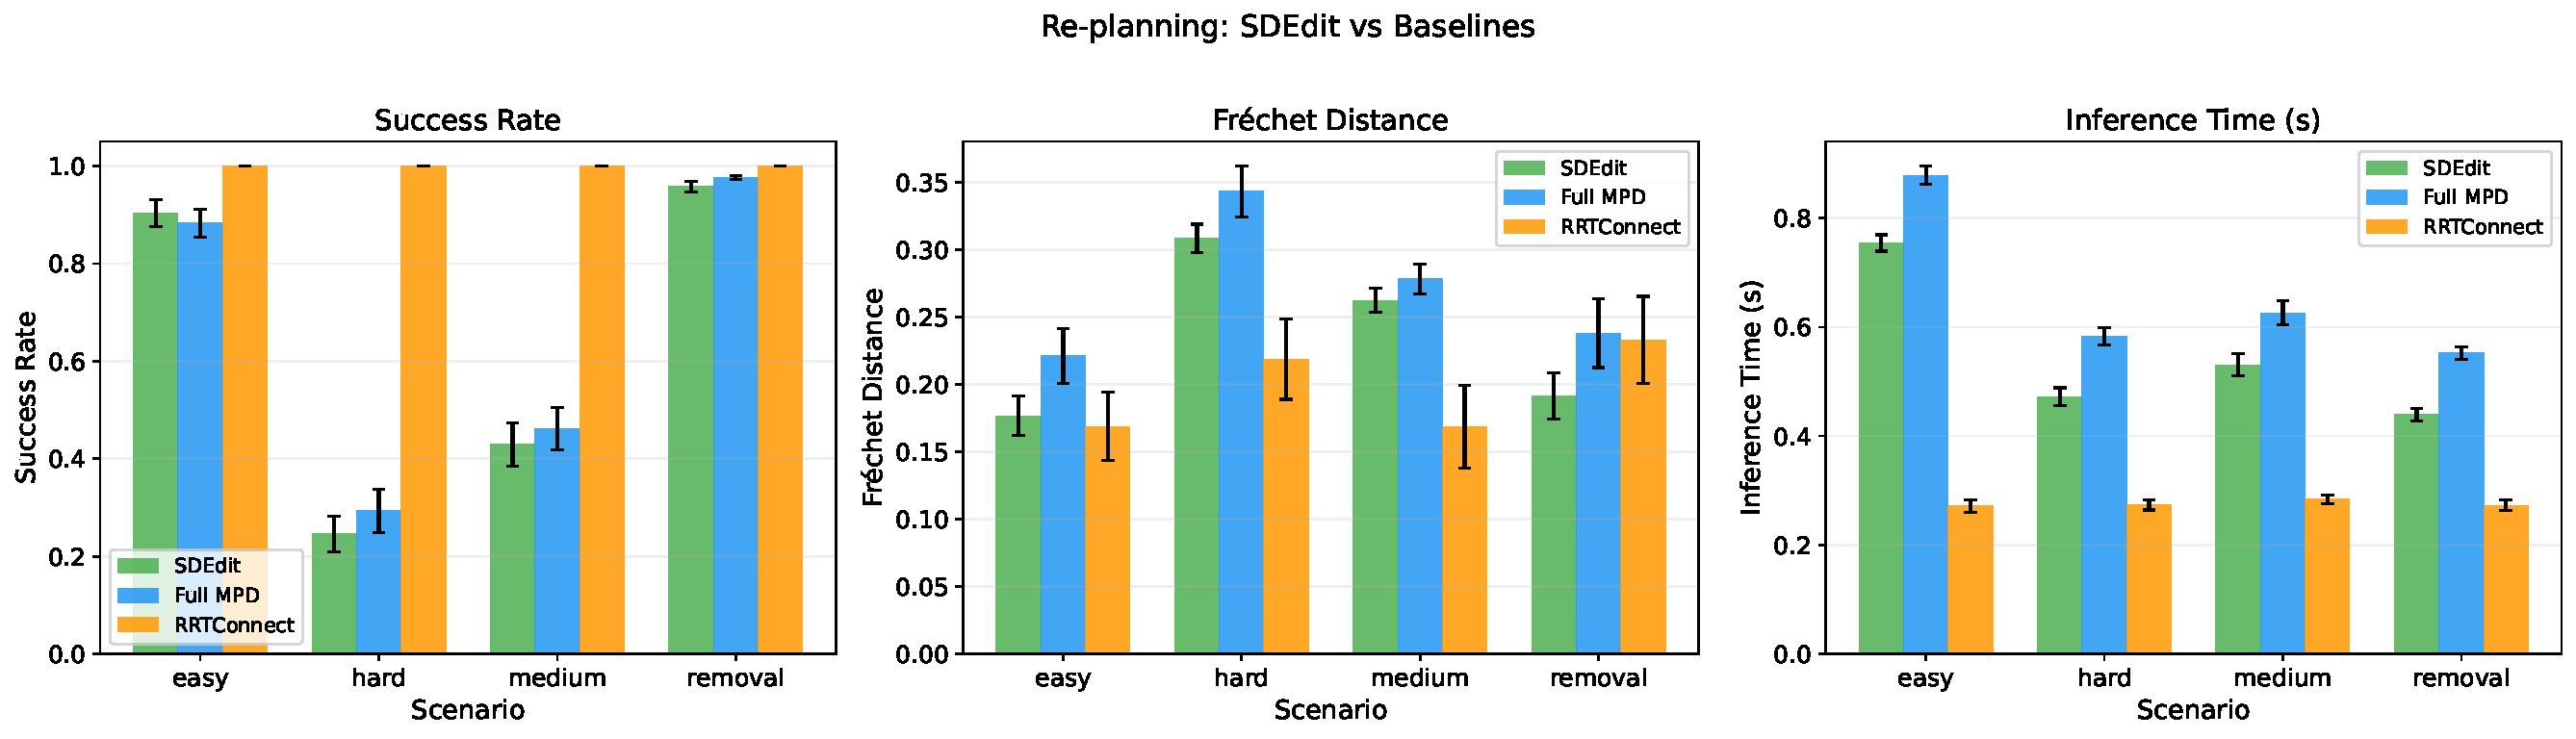
\includegraphics[width=0.9\linewidth]{../scripts/inference/logs_experiments/figures/fig_baselines_comparison.pdf}
  \placeholder{1cm}{Figure~3: Grouped bar chart comparing success rates of
    SDEdit, Full MPD, and RRTConnect across the four scenarios.}
  \caption{Success-rate comparison across difficulty scenarios.}
  \label{fig:baselines_bar}
\end{figure}

\subsection{Experiment 3: Inference Speed}
\label{sec:exp_speed}

Figure~\ref{fig:speed} reports wall-clock inference time as a function
of~$t_0$.  Because SDEdit denoises from $t_0$ rather than the full schedule,
lower noise levels yield proportionally faster inference.  At $t_0{=}1$
MPEdit is roughly $2\times$ faster than Full MPD.

\begin{figure}[t]
  \centering
  % Replace with: 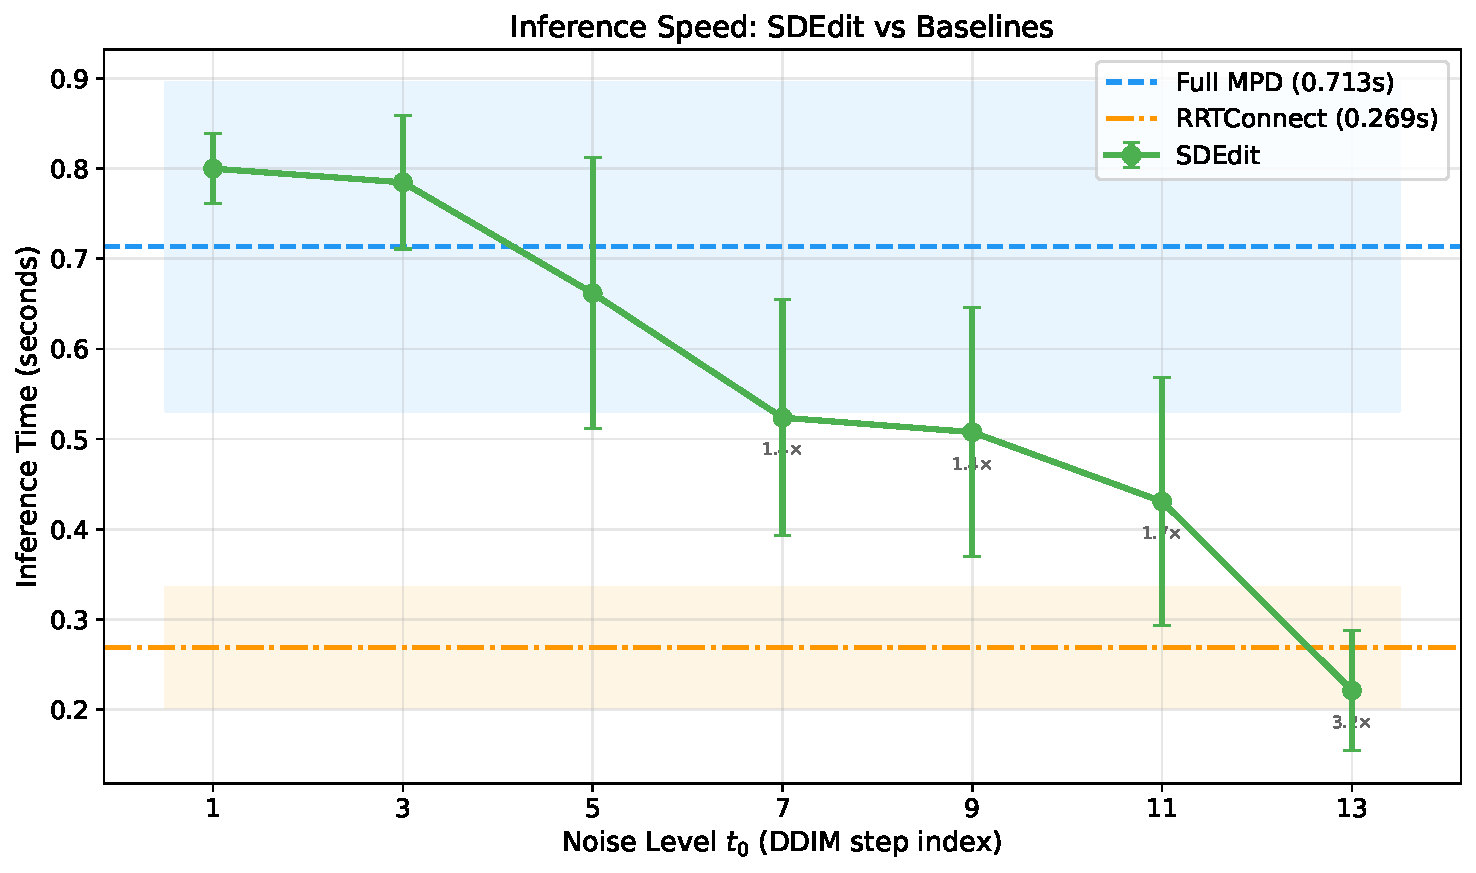
\includegraphics[width=\linewidth]{../scripts/inference/logs_experiments/figures/fig5_speed.pdf}
  \placeholder{1cm}{Figure~4: Inference time (seconds) vs.\ noise level
    $t_0$.  SDEdit at low $t_0$ is faster than Full MPD.}
  \caption{Inference speed vs.\ noise level.}
  \label{fig:speed}
\end{figure}

\subsection{Experiment 4: Output Diversity}
\label{sec:exp_diversity}

Figure~\ref{fig:diversity} shows the mean pairwise Fréchet distance among the
100 generated trajectories per start--goal pair.  Higher noise levels produce
more diverse outputs; at $t_0{=}1$ the outputs are nearly identical to the
input, while at $t_0{=}13$ diversity approaches that of Full MPD.

\begin{figure}[t]
  \centering
  % Replace with: 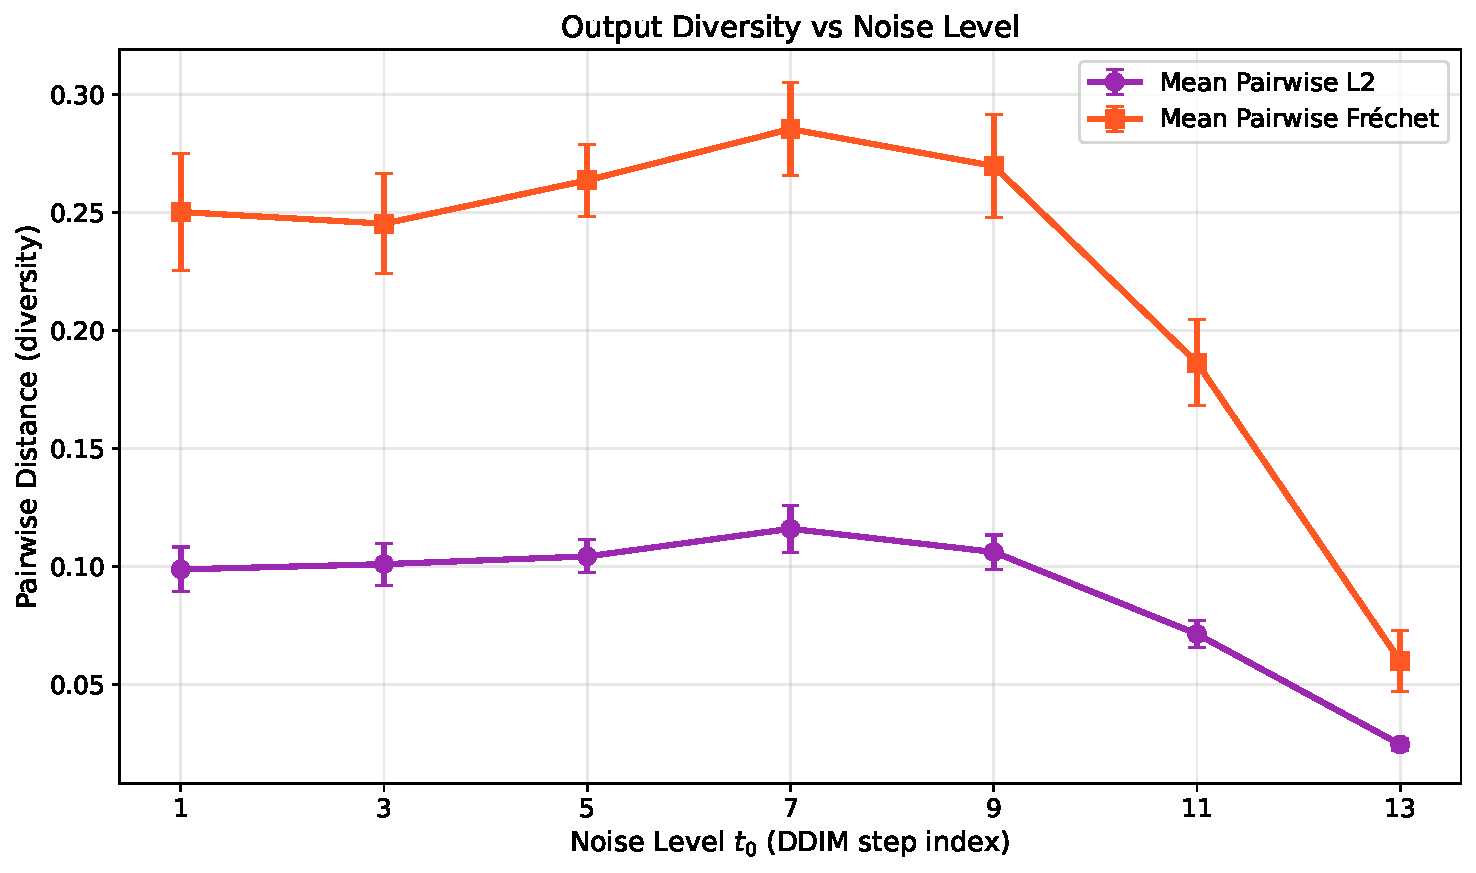
\includegraphics[width=\linewidth]{../scripts/inference/logs_experiments/figures/fig6_diversity.pdf}
  \placeholder{1cm}{Figure~5: Pairwise trajectory diversity (Fréchet
    distance) vs.\ noise level $t_0$.}
  \caption{Output diversity vs.\ noise level.}
  \label{fig:diversity}
\end{figure}

% ══════════════════════════════════════════════════════════════════════════════
\section{Discussion}
\label{sec:discussion}
% ══════════════════════════════════════════════════════════════════════════════

\paragraph{When does MPEdit help?}
MPEdit is most effective when the environment change is \emph{local}: adding
or removing a small obstacle leaves most of the original path valid, and a
moderate noise level ($t_0 \approx 7$) suffices to re-route.  In easy and
removal scenarios, MPEdit matches or exceeds Full MPD in both success rate
and faithfulness.

\paragraph{Limitations.}
When the topology of free space changes drastically (hard scenario), cost
guidance is insufficient to escape the basin of the reference path.
Classical planners like RRTConnect handle such cases far more reliably.
A hybrid strategy---detecting large changes and falling back to RRT---is a
natural extension.

\paragraph{Sketch mode.}
The sketch-to-path pipeline (Appendix~\ref{app:sketch}) works well in 2-D
but is less practical for high-DOF robots where joint-space sketching is
unintuitive.  Extending it to task-space end-effector paths via inverse
kinematics is a promising direction.

% ══════════════════════════════════════════════════════════════════════════════
\section{Conclusions}
\label{sec:conclusions}
% ══════════════════════════════════════════════════════════════════════════════

We presented MPEdit, a simple yet effective method for adapting
diffusion-based motion planning to dynamic environments by borrowing the
SDEdit principle.  By noising an existing trajectory to an intermediate
diffusion step and denoising with an updated collision-cost guide, MPEdit
produces paths that are faithful to the original route while avoiding new
obstacles.  Our experiments demonstrate clear trade-offs controlled by the
noise level~$t_0$ and confirm that MPEdit is competitive with full
re-planning in success rate while offering superior path faithfulness and
practical speed-ups.

The framework is implemented in Python using PyTorch and is fully
reproducible via provided configuration files and scripts.  All code,
pre-trained models, and experiment configurations are available in the
project repository.

% ══════════════════════════════════════════════════════════════════════════════
% REFERENCES
% ══════════════════════════════════════════════════════════════════════════════

\bibliographystyle{plainnat}

\begin{thebibliography}{10}

\bibitem{carvalho2023mpd}
J.~Carvalho, A.~T. Le, M.~Baierl, D.~Koert, and J.~Peters.
\newblock Motion planning diffusion: Learning and planning of robot motions
  with diffusion models.
\newblock \emph{arXiv preprint arXiv:2308.01557}, 2023.

\bibitem{meng2022sdedit}
C.~Meng, Y.~He, Y.~Song, J.~Song, J.~Wu, J.-Y. Zhu, and S.~Ermon.
\newblock {SDEdit}: Guided image synthesis and editing with stochastic
  differential equations.
\newblock In \emph{International Conference on Learning Representations
  (ICLR)}, 2022.

\bibitem{lavalle1998rrt}
S.~M. LaValle.
\newblock Rapidly-exploring random trees: A new tool for path planning.
\newblock Technical Report TR 98-11, Computer Science Dept., Iowa State
  University, 1998.

\bibitem{kuffner2000rrtconnect}
J.~J. Kuffner and S.~M. LaValle.
\newblock {RRT-Connect}: An efficient approach to single-query path planning.
\newblock In \emph{IEEE International Conference on Robotics and Automation
  (ICRA)}, pages 995--1001, 2000.

\bibitem{song2021ddim}
J.~Song, C.~Meng, and S.~Ermon.
\newblock Denoising diffusion implicit models.
\newblock In \emph{International Conference on Learning Representations
  (ICLR)}, 2021.

\bibitem{dhariwal2021diffusion}
P.~Dhariwal and A.~Nichol.
\newblock Diffusion models beat {GANs} on image synthesis.
\newblock In \emph{Advances in Neural Information Processing Systems
  (NeurIPS)}, 2021.

\bibitem{ho2020ddpm}
J.~Ho, A.~Jain, and P.~Abbeel.
\newblock Denoising diffusion probabilistic models.
\newblock In \emph{Advances in Neural Information Processing Systems
  (NeurIPS)}, 2020.

\bibitem{janner2022diffuser}
M.~Janner, Y.~Du, J.~Tenenbaum, and S.~Levine.
\newblock Planning with diffusion for flexible behavior synthesis.
\newblock In \emph{International Conference on Machine Learning (ICML)}, 2022.

\bibitem{urain2023se3difffields}
J.~Urain, N.~Funk, J.~Peters, and G.~Chalvatzaki.
\newblock {SE(3)-DiffusionFields}: Learning smooth cost functions for joint
  grasp and motion optimization through diffusion.
\newblock In \emph{IEEE International Conference on Robotics and Automation
  (ICRA)}, 2023.

\end{thebibliography}

% ══════════════════════════════════════════════════════════════════════════════
% APPENDIX
% ══════════════════════════════════════════════════════════════════════════════
\clearpage
\appendix

\section{Sketch-to-Path Mode}
\label{app:sketch}

The sketch-to-path mode allows a user to provide a rough, hand-drawn
trajectory that is refined by the diffusion model into a collision-free,
smooth path.  This appendix describes the interactive tool and presents
qualitative results.

\subsection{Interactive Path Sketcher}

The \texttt{PathSketcher} GUI (Figure~\ref{fig:sketcher_ui}) renders the 2-D
obstacle map and lets the user draw a freehand curve from start to goal.
Upon mouse release the raw sketch is processed:
\begin{enumerate}
  \item Near-duplicate points are removed.
  \item A cubic B-spline is fitted with smoothing parameter $s = 0.001$.
  \item The spline is resampled to $T$ waypoints to match the model input.
  \item Endpoints are snapped exactly to the start and goal configurations.
\end{enumerate}
The resulting sketch is displayed in green; the user can clear and redraw
before confirming.

\begin{figure}[H]
  \centering
  % Replace with a screenshot of the PathSketcher GUI
  \placeholder{3cm}{Screenshot of the PathSketcher interactive GUI showing
    the 2-D obstacle map, start/goal markers, the raw orange sketch, and
    the resampled green path.}
  \caption{PathSketcher interactive GUI.  The user draws a freehand path
    (orange) which is smoothed and resampled (green).}
  \label{fig:sketcher_ui}
\end{figure}

\subsection{Sketch Experiment: Corruption vs.\ Noise Level}

In the sketch experiment, we systematically vary two parameters:
\begin{itemize}
  \item \textbf{Corruption level $\sigma$:} Gaussian noise added to a
    ground-truth path to simulate sketches of varying quality
    ($\sigma \in \{0.05, 0.10, 0.15, 0.20, 0.25, 0.30\}$).
  \item \textbf{Noise level $t_0$:} the SDEdit diffusion starting step
    ($t_0 \in \{1, 3, 5, 7, 9, 11, 13\}$).
\end{itemize}
Figure~\ref{fig:sketch_heatmap} shows the resulting heatmap of success rate
and faithfulness (Fréchet distance) over the $(\sigma, t_0)$ grid.

\begin{figure}[H]
  \centering
  % Replace with: 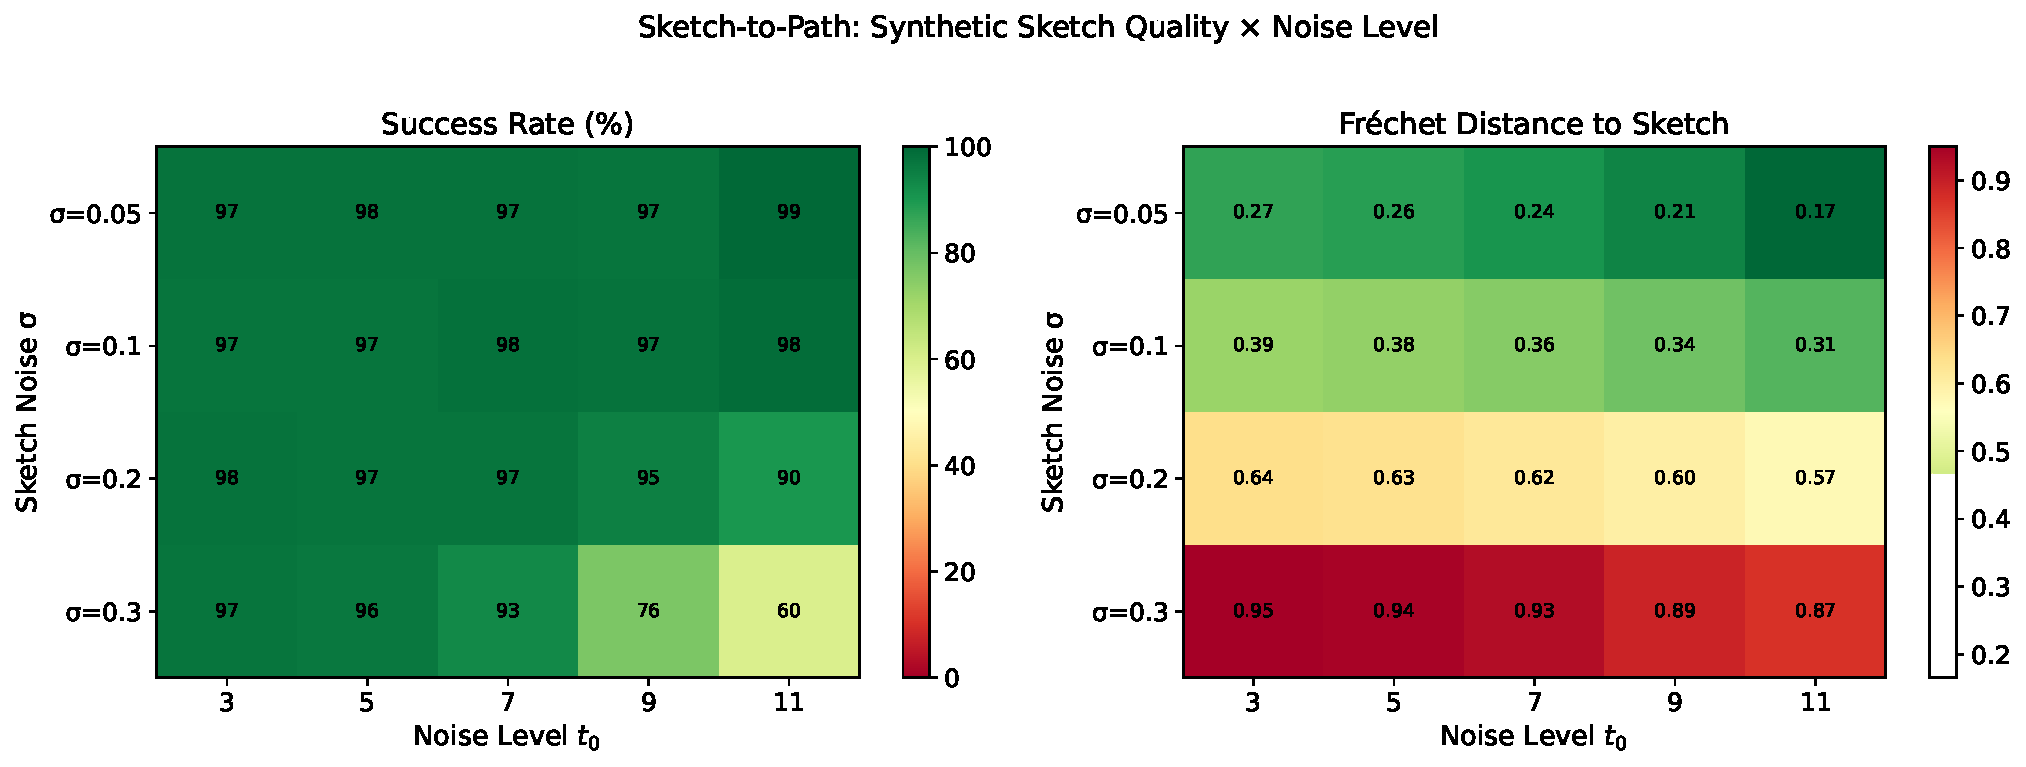
\includegraphics[width=\linewidth]{../scripts/inference/logs_experiments/figures/fig4_sketch_heatmap.pdf}
  \placeholder{3cm}{Figure: Heatmap of success rate and Fréchet distance
    over corruption level $\sigma$ (x-axis) and noise level $t_0$ (y-axis).
    Darker regions indicate better performance.}
  \caption{Sketch-mode heatmap.  Each cell shows the success rate and mean
    Fréchet distance for a given $(\sigma, t_0)$ combination.}
  \label{fig:sketch_heatmap}
\end{figure}

\subsection{Qualitative Sketch Examples}

Below are placeholder panels showing representative sketch-to-path results:

\begin{figure}[H]
  \centering
  % Replace with actual sketch-to-path result images
  \placeholder{3cm}{Panel (a): Low corruption ($\sigma{=}0.05$), low noise
    ($t_0{=}3$).  The output closely follows the sketch.\\[4pt]
    Panel (b): High corruption ($\sigma{=}0.25$), moderate noise
    ($t_0{=}7$).  The model smooths out the sketch and avoids obstacles.\\[4pt]
    Panel (c): Hand-drawn sketch via the GUI, refined by MPEdit.}
  \caption{Sketch-to-path examples.  (a)~Low corruption, low noise.
    (b)~High corruption, moderate noise.
    (c)~Freehand GUI sketch refined by MPEdit.}
  \label{fig:sketch_examples}
\end{figure}

\section{Before-and-After Visualizations}
\label{app:before_after}

The following placeholders show the three-panel before/after visualization
generated by MPEdit's plotting utilities: the original environment with the
reference path, the modified obstacle map, and the regenerated trajectories.

\begin{figure}[H]
  \centering
  % Replace with actual before-after images from sdedit_before_after-*.png outputs
  \placeholder{3cm}{Three-panel figure:\\
    \textbf{Left:} Original obstacles + reference path (blue dashed).\\
    \textbf{Center:} Modified obstacles (new obstacle highlighted in red).\\
    \textbf{Right:} Regenerated paths (orange semi-transparent) + best path
    (green solid).}
  \caption{Before-and-after re-planning visualization.}
  \label{fig:before_after}
\end{figure}

\section{Implementation and Usage}
\label{app:implementation}

The project is implemented in Python using PyTorch.  Key commands:

\begin{verbatim}
# Activate environment
source set_env_variables.sh
conda activate mpd-splines-public

# Run batch SDEdit inference (re-planning)
cd scripts/inference
python inference_sdedit.py

# Run interactive SDEdit with GUI
python inference_sdedit_interactive.py --sdedit_mode replan

# Run sketch mode
python inference_sdedit_interactive.py --sdedit_mode sketch

# Run full experiment suite
python ../experiments/run_experiment.py \
    --config ../experiments/cfgs/experiment_2d.yaml

# Plot experiment results
python ../experiments/plot_results.py \
    --results_dir logs_experiments
\end{verbatim}

All experiment configurations are stored in YAML files under
\texttt{scripts/experiments/cfgs/} and
\texttt{scripts/inference/logs\_experiments/experiment\_config.yaml}.

\end{document}
